\subsection{B-Scan}
\label{sec:bscana}
Die gemessene Tiefe beim B-Scan ist
\begin{equation}
    h_\text{B-Scan}= \SI{80.66}{\milli\meter}\:.
\end{equation}
Die Werte der jeweiligen Störstelle stammen aus den Abbildungen \ref{fig:bscano} und \ref{fig:bscanu}.
Bei diesen wurde die Farbe invertiert um Tinte zu sparen.
Die Rechnung verläuft analog zu der beim A-Scan, Kapitel \ref{sec:ascana}.
Die Ergebnisse stehen auch in Kapitel \ref{sec:tabellen}, Tabelle \ref{tab:scana}.

\begin{figure}
    \centering
    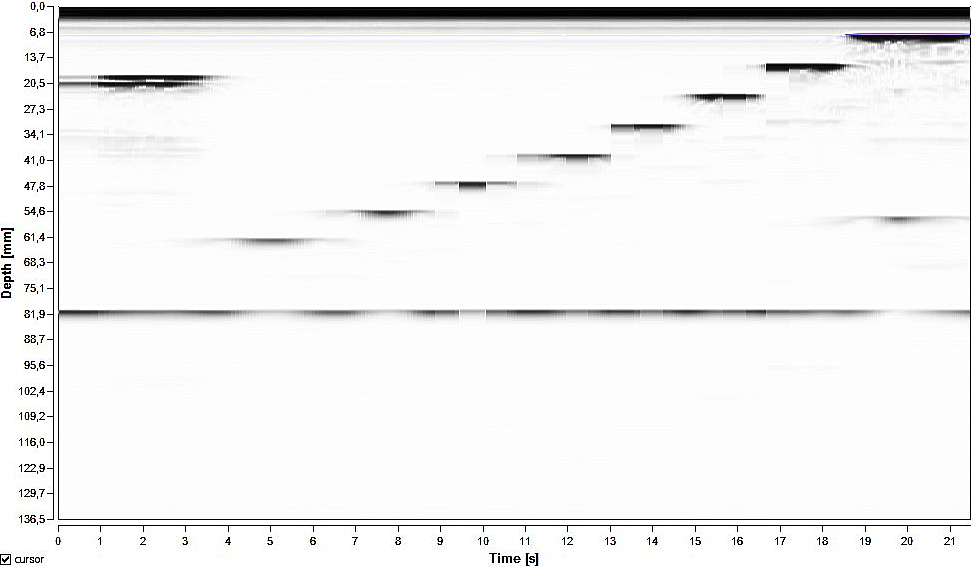
\includegraphics[width=\textwidth]{content/bilder/b-scan-oben.jpg}
    \caption{B-Scan von oben.}
    \label{fig:bscano}
\end{figure}

\begin{figure}
    \centering
    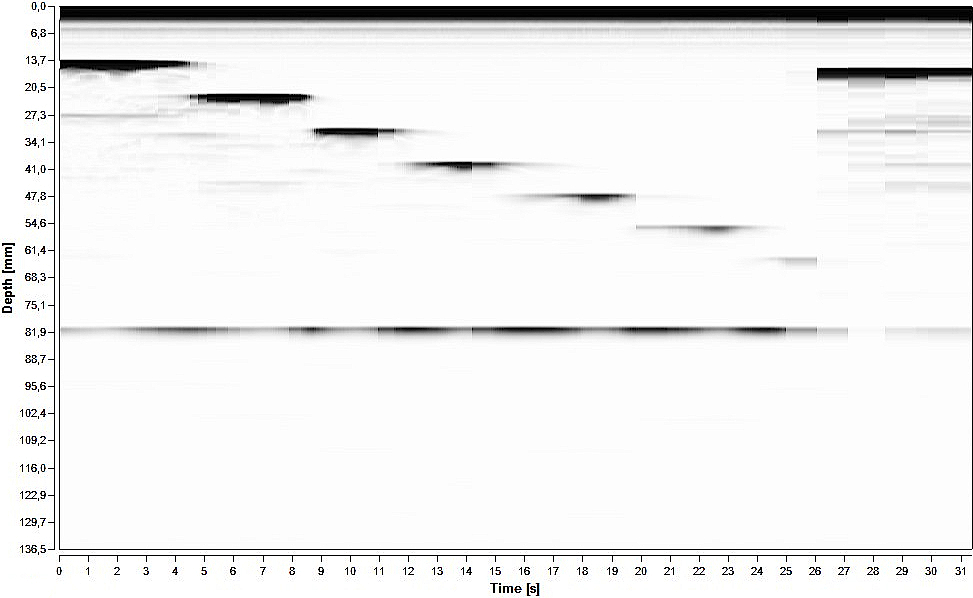
\includegraphics[width=\textwidth]{content/bilder/b-scan-unten.jpg}
    \caption{B-Scan von unten.}
    \label{fig:bscanu}
\end{figure}
